%\documentclass{article}
\documentclass[11pt]{article}
\usepackage[top=56pt,bottom=58pt,left=50pt,right=48pt]{geometry}

\usepackage[slovene]{babel}
\usepackage{amsmath}
\usepackage{color}
%\usepackage{graphicx,subfigure}

%\usepackage{subfigure}

\usepackage[T1]{fontenc}
\usepackage[utf8]{inputenc}
\usepackage{lmodern}
\usepackage{amsmath}
\usepackage{tikz}
\usetikzlibrary{shapes,shapes.geometric,arrows,fit,calc,positioning,automata}

\usepackage{amsfonts}
\usepackage{mathrsfs}

\usepackage{float}

\usepackage{caption}
\usepackage{subcaption}

\usepackage{enumerate}

%\usepackage{natbib}

%\usepackage{chemformula}
%\usepackage[version=4]{mhchem}
%\usepackage{mychemistry}
%\usepackage{chemfig}

%\def\phi{\varphi}
%\def\eps{\varepsilon}
%\def\theta{\vartheta}

%\usepackage{physics} ta je za vektorje: \vectorbold{}

\newcommand{\thisyear}{2020/21}

\renewcommand{\Re}{\mathop{\rm Re}\nolimits}
\renewcommand{\Im}{\mathop{\rm Im}\nolimits}
\newcommand{\Tr}{\mathop{\rm Tr}\nolimits}
\newcommand{\diag}{\mathop{\rm diag}\nolimits}
\newcommand{\dd}{\,\mathrm{d}}
\newcommand{\ddd}{\mathrm{d}}
\newcommand{\ii}{\mathrm{i}}
\newcommand{\lag}{\mathcal{L}\!}
\newcommand{\ham}{\mathcal{H}\!}
\newcommand{\four}[1]{\mathcal{F}\!\left(#1\right)}
\newcommand{\bigO}[1]{\mathcal{O}\!\left(#1\right)}
\newcommand{\sh}{\mathop{\rm sinh}\nolimits}
\newcommand{\ch}{\mathop{\rm cosh}\nolimits}
\renewcommand{\th}{\mathop{\rm tanh}\nolimits}
\newcommand{\erf}{\mathop{\rm erf}\nolimits}
\newcommand{\erfc}{\mathop{\rm erfc}\nolimits}
\newcommand{\sinc}{\mathop{\rm sinc}\nolimits}
\newcommand{\rect}{\mathop{\rm rect}\nolimits}
\newcommand{\ee}[1]{\cdot 10^{#1}}
\newcommand{\inv}[1]{\left(#1\right)^{-1}}
\newcommand{\invf}[1]{\frac{1}{#1}}
\newcommand{\sqr}[1]{\left(#1\right)^2}
\newcommand{\half}{\frac{1}{2}}
\newcommand{\thalf}{\tfrac{1}{2}}
\newcommand{\pd}{\partial}
\newcommand{\Dd}[3][{}]{\frac{\ddd^{#1} #2}{\ddd #3^{#1}}}
%\newcommand{\Pd}[3][{}]{\frac{\pd^{#1} #2}{\pd #3^{#1}}}
\newcommand{\avg}[1]{\left\langle#1\right\rangle}
\newcommand{\norm}[1]{\left\Vert #1 \right\Vert}
\newcommand{\braket}[2]{\left\langle #1 \vert#2 \right\rangle}
%\newcommand{\obraket}[3]{\left\langle #1 \vert #2 \vert #3 \right \rangle}
%\newcommand{\hex}[1]{\texttt{0x#1}}
\newcommand{\vect}[1]{\boldsymbol{#1}}

\renewcommand{\iint}{\mathop{\int\mkern-13mu\int}}
\renewcommand{\iiint}{\mathop{\int\mkern-13mu\int\mkern-13mu\int}}
\newcommand{\oiint}{\mathop{{\int\mkern-15mu\int}\mkern-21mu\raisebox{0.3ex}{$\bigcirc$}}}

\newcommand{\wunderbrace}[2]{\vphantom{#1}\smash{\underbrace{#1}_{#2}}}

\renewcommand{\vec}[1]{\overset{\smash{\hbox{\raise -0.42ex\hbox{$\scriptscriptstyle\rightharpoonup$}}}}{#1}}
\newcommand{\bec}[1]{\mathbf{#1}}
\newcommand{\q}[1]{``#1''}



\begin{document}


\begin{titlepage}
\begin{center}
	
	{\sc\Large	Teorija dinamičnih sistemov}\\
	\vspace*{5cm}
	\LARGE\textbf{Naloga 25: Sinajev biljard}\\
	\vspace{0.2cm}
	\vspace{1.6cm}
	\large{Avtor: Žan Butala}\\
	\text{vpisna številka: 28222060}
 
      % \vspace{1cm}
	%\begin{figure}[H]
   %	 \centering
    %	\includegraphics[width=10cm]{semafor1.png}
    	%\label{fig:graf1}
	%\end{figure}

       \vspace{5cm}



       \vfill

	\normalsize
 
       {\sc 18. januar 2024\\
	\vspace{0.2cm}
       Univerza v Ljubljani\\
       Fakulteta za matematiko in fiziko\\}
      
\end{center}
\end{titlepage}


\newpage

\section{Naloga:}
Izračunaj Ljapunove eksponente za Sinajev biljard v obliki enotskega kvadrata, ki ima v centru krožno oviro s polmerom $R < 1/2$.
Ali lahko kvaliltativno razložiš rezultate? Nariši nekaj kratkih periodičnih orbit in analitično izračunaj stabilnostne eksponente.






\vspace*{2cm}

\section{Ljapunovi eksponenti}
Nalogo sem začel s preprosto simulacijo Sinajevega biljarda.
Ker je gibanje med odboji premoenakomerno, iteracije izvajal kar z Eulerjevo metodo, kjer je bila velikost hitrosti 1, dolžina časovnega koraka pa $dt =10^{-3}$.
Na vsakem koraku sem preveril, če je točka zunaj kvadrata ali znotraj kroga ter v tem primeru prezrcalil vektor hitrosti.
Pri odboju od stranic kvadrata je to super enostavno, na krogu pa sem si pomagal s funkcijo \texttt{arctan2()}, ki vrača vrednosti med $-\pi$ in $\pi$.
Točko trka sem s tem prepisal v \q{polarne koordinate}, nato sem lahko zračunal vpadni k\'ot in vektor hitrosti ustrezno prezrcalil.


\begin{figure}[H]
       \centering
       \hspace*{-0mm}
       
\includegraphics[width=10cm]{ljapun01.png}
       \caption{Vsakih 500 korakov reskalacija na $\varepsilon$-oddaljenost.}
       \label{fig:}
\end{figure}

Na predavanjih smo povedali, da v praksi osnovna formula za Ljapunov eksponent ni dobra, ker zaradi numerike ne moremo dovolj dobro izvesti limite $\delta \rightarrow 0$.
Izraz smo predelali v obliko
\begin{equation}
\lambda = \lim_{t \rightarrow \infty} \frac{1}{t} \bigg (\sum_i \ln \frac{|\delta(t_i)|}{\varepsilon} \bigg ),
\end{equation}
kjer je $\delta(t_i)$ oddaljenost dveh nekdaj bližnjih točk.
Reskalacijo na razdaljo $\varepsilon = 10^{-6}$ sem izvedel vsakih 500 korakov, in z množico razdalj $\{\delta_i\}$ dobil približek Ljapunovega eksponenta.
Postopek sem ponovil za različne vrednosti polmera $R$.
\begin{figure}[H]
       \centering
       \hspace*{-0mm}
       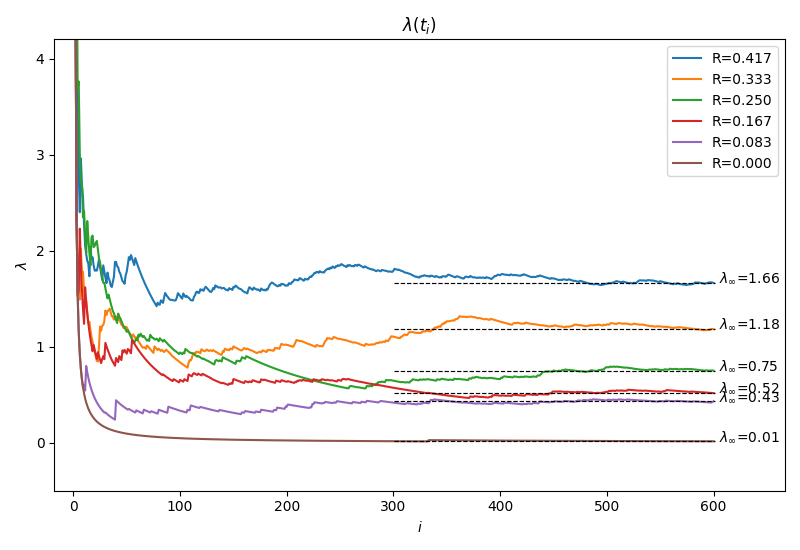
\includegraphics[width=10cm]{ljapun02b.png}
       \caption{Konvergenca Ljapunovih eksponentov za različne $R$.}
       \label{fig:}
\end{figure}
Začetni zamik opazovane orbite glede na referenčno sem žrebal naključno iz kroga z radijem $\varepsilon$.
Zato sem vsakič, ko sem ponovno pognal program, dobil nekoliko drugačno vrednost $\lambda$ za isti $R$.
Algoritem sem popravil na premik opazovane orbite pravokotno na vektor hitrosti, kar je prineslo k manjši raztresenosti točk pri danem $R$.
Na koncu sem to še dodatno izboljšal s povečanjem števila iteracij.
$R$ sem pustil teči tudi čez $1/2$, kar pomeni, da je bil delec takrat ujet v okolico enega od ogljišč.
\begin{figure}[H]
       \centering
       \begin{subfigure}[b]{0.49\textwidth}
          \hspace*{-1mm}
           \centering
           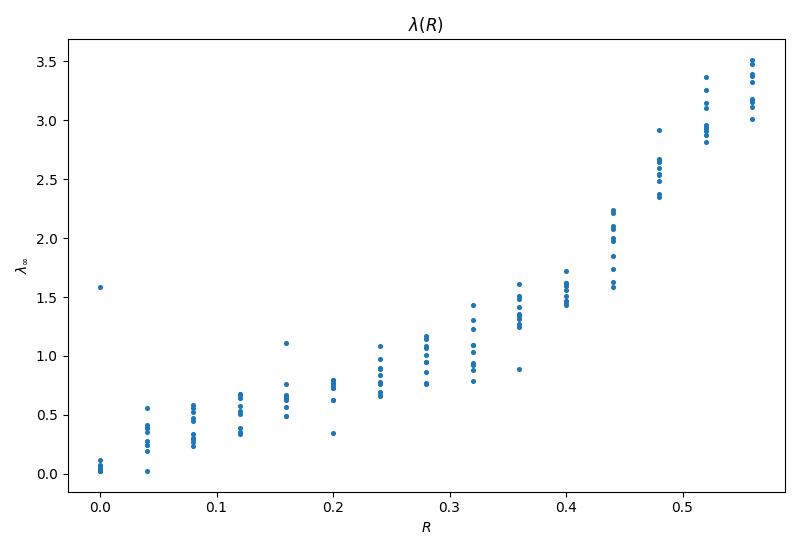
\includegraphics[width=1.\textwidth]{ljapun04b.png}
           %\caption{$R=3/8$.}
           \label{fig:pot1a}
       \end{subfigure}
       \begin{subfigure}[b]{0.49\textwidth}
         \hspace*{0mm}
           \centering
           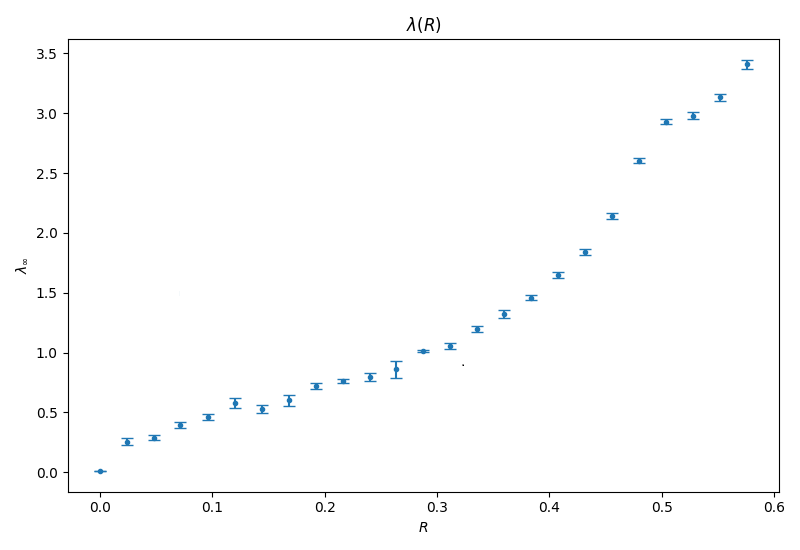
\includegraphics[width=1.\textwidth]{ljapun04c_1.png}
           %\caption{$R=2/8$.}
           \label{fig:pot1b}
       \end{subfigure}
          \caption{Odvisnost Ljapunovega eksponenta od polmera $R$.}
          \label{fig:}
\end{figure}


\newpage
\section{Stabilnost periodičnih orbit}
\subsection*{Fazni portreti v Poincre-Birchoffovih koordinatah}
V drugem delu sem obravnaval periodične trajektorije in njih stabilnost.
Nekaj primekrov najdemo, če narišemo fazne portrete v Poincare-Birchoffovih koordinatah $(s,p_s)$, kjer je $s$ ločna dolžina roba, $p_s$ pa tangentna komponenta hitrosti pri odboju.
Dolžino sem začel meriti v desnem spodnjem vogalu v pozitivni matematični smeri.
Ko sem prišel okrog, sem nadaljeval še na krogu, zato je parameter $s$ teče med 0 in $4 + 2\pi R$.
To morda ni najboljše, ker vrednosti $s=0$ in $s=4$ predstavljata isto točko na kvadratu, $s=4+\epsilon$ pa je točka na krogu (matematiki bi rekli, da območje ni enostavno povezano).
Fazni prostor v taki obliki je torej iz dveh ločenih delov.
\begin{figure}[H]
       \centering
       \begin{subfigure}[b]{0.49\textwidth}
           \hspace*{-1mm}
           \centering
           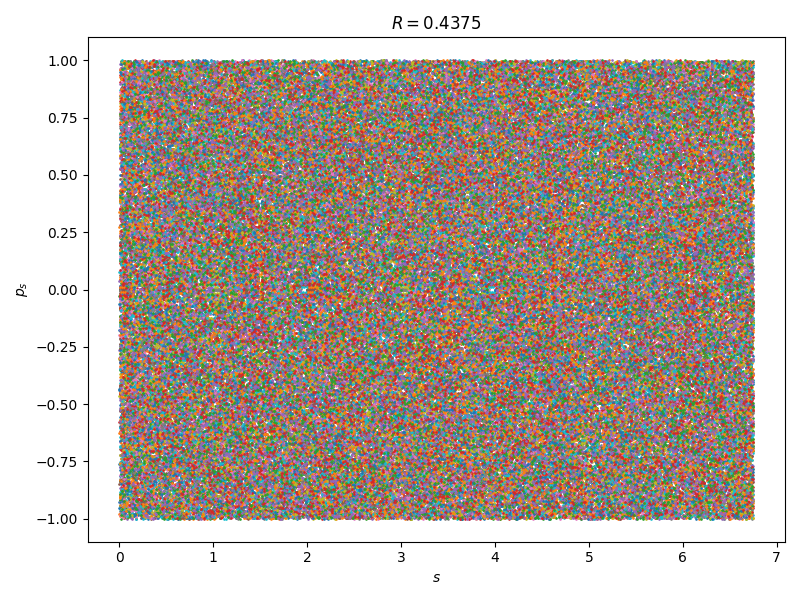
\includegraphics[width=1.\textwidth]{poincare04a.png}
           %\caption{$R=3/8$.}
           \label{fig:pot1a}
       \end{subfigure}
       \begin{subfigure}[b]{0.49\textwidth}
           \hspace*{0mm}
           \centering
           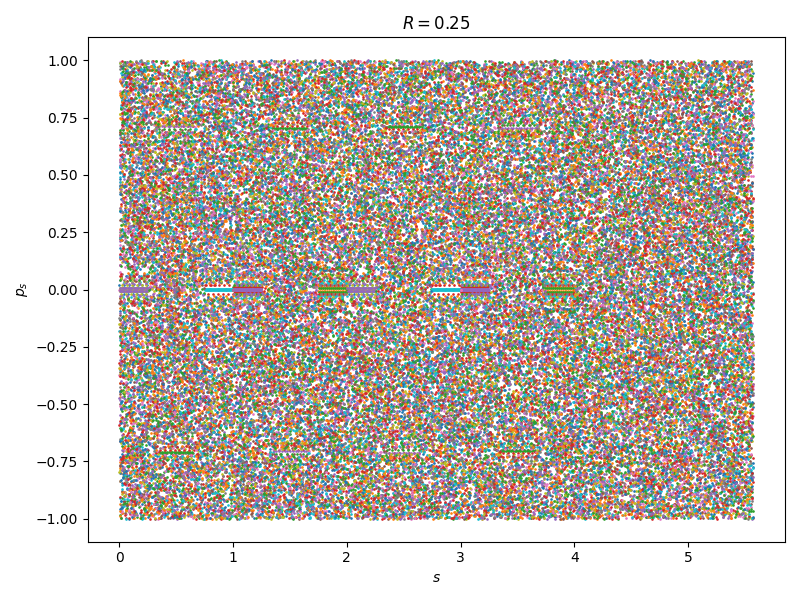
\includegraphics[width=1.\textwidth]{poincare04b.png}
           %\caption{$R=2/8$.}
           \label{fig:pot1b}
       \end{subfigure}
       \begin{subfigure}[b]{0.49\textwidth}
              \hspace*{-1mm}
              \centering
              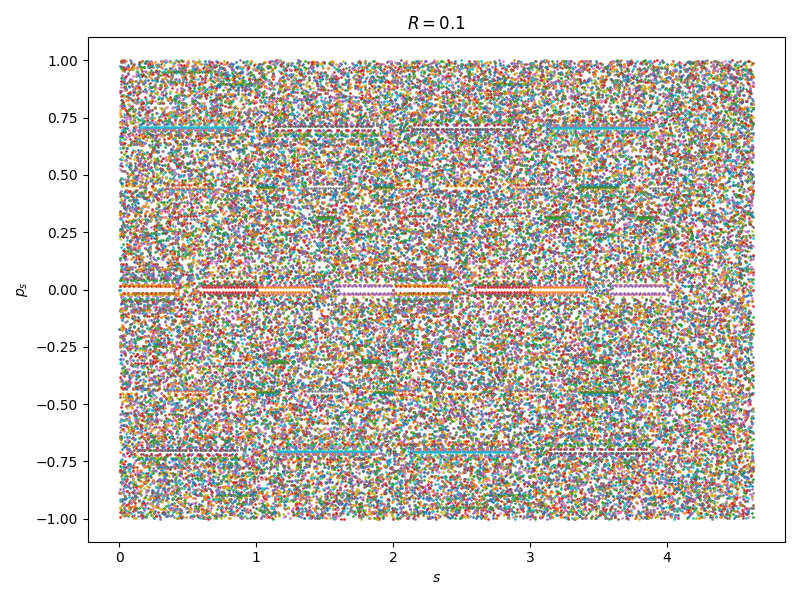
\includegraphics[width=1.\textwidth]{poincare04c.png}
              %\caption{$R=3/8$.}
              \label{fig:pot1a}
       \end{subfigure}
       \begin{subfigure}[b]{0.49\textwidth}
              \hspace*{0mm}
              \centering
              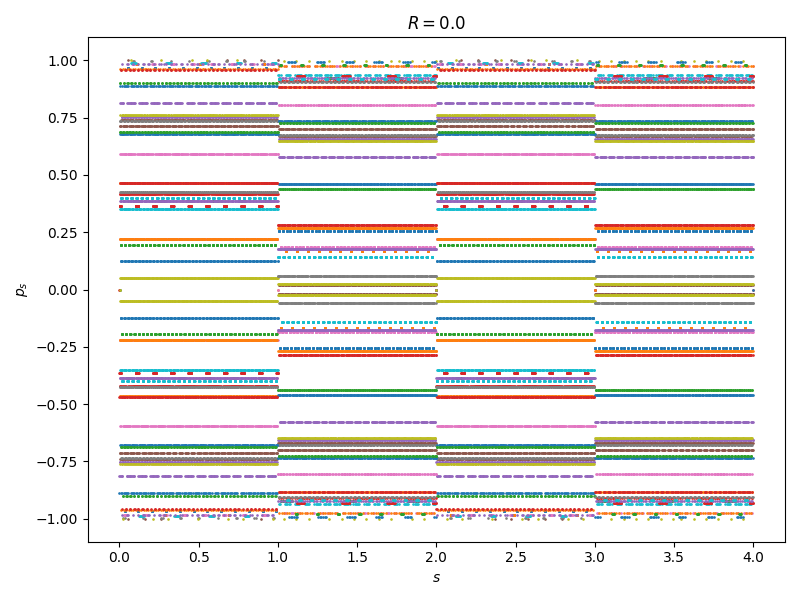
\includegraphics[width=1.\textwidth]{poincare04d.png}
              %\caption{$R=2/8$.}
              \label{fig:pot1b}
       \end{subfigure}
          \caption{Poincarejeve sečne ploskve za Sinajev biljard. Vsaka slika sestoji iz 30 trajektorij, }
          \label{fig:poinc}
\end{figure}
Ko gre $R$ proti $1/2$ dobimo globalni kaos, z zmanjševanjem pa se začnejo pojavljati ekvivalenti stabilnostnih otočkov.
Pri $R=0$ dobimo pričakovano sliko integrabilnega kvadratnega biljarda.

\subsection*{Stabilnost}
Na predavanjih smo za $z, \theta \ll 1$ zapisali prehodno matriko za prosti let in odboj
\begin{equation}
\begin{split}
\begin{bmatrix}
z' \\
\theta'
\end{bmatrix}
 = &
F_{odboj} F_{prost}
\begin{bmatrix}
z \\
\theta
\end{bmatrix} \\
F_{odboj} &=
\begin{bmatrix}
-1 & 0\\
\frac{2}{\rho \cos \psi} & -1
\end{bmatrix} \\
F_{prost} &=
\begin{bmatrix}
1 & l\\
0 & 1
\end{bmatrix}
\end{split}
\end{equation}
ter pogoj za stabilnost
\begin{equation}
-2 \le \text{tr} F \le 2.
\end{equation}
Na koncu sem poračunal matriko $F$ in njeno sled za 4 očitne tipe periodičnih trajektorij.
Ugotovil sem, da stabilnostnemu kriteriju zadoščajo tiste, ki jih lahko najdemo na faznih portretih (vodoravne črtice na sliki \ref{fig:poinc}).
Nestabilne je potrebno uganiti.
\begin{itemize}
\item $\psi_{1,2} = 0$, $\rho_{1,2} = \infty$
\begin{figure}[H]
       \centering
       \hspace*{-0mm}
       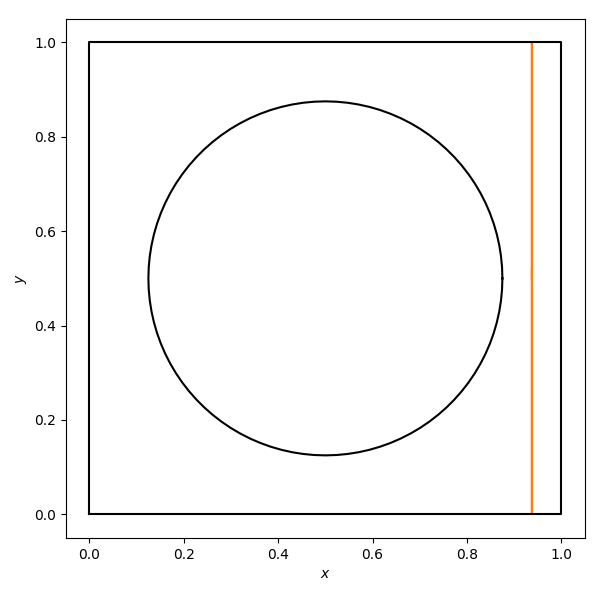
\includegraphics[width=5cm]{sinai2a.png}
       %\caption{Bouncing ball 1.}
       \label{fig:}
\end{figure}
\begin{equation}
\begin{split}
F =& F_{odb_2} F_{prost_2} F_{odb_1} F_{prost_1} \\
 =& 
\begin{bmatrix}
-1 & 0\\
0 & -1
\end{bmatrix}
\begin{bmatrix}
1 & l\\
0 & 1
\end{bmatrix}
\begin{bmatrix}
-1 & 0\\
0 & -1
\end{bmatrix}
\begin{bmatrix}
1 & l\\
0 & 1
\end{bmatrix} \\
=&
\begin{bmatrix}
1 &2 l\\
0 & 1
\end{bmatrix}
\end{split}
\end{equation}

\begin{equation}
\text{tr}F = 2
\end{equation}



\item $\psi = 0$, $\rho_2 = -R$
\begin{figure}[H]
\hspace*{18mm}
       \begin{subfigure}[b]{0.32\textwidth}
          \hspace*{0mm}
           \centering
           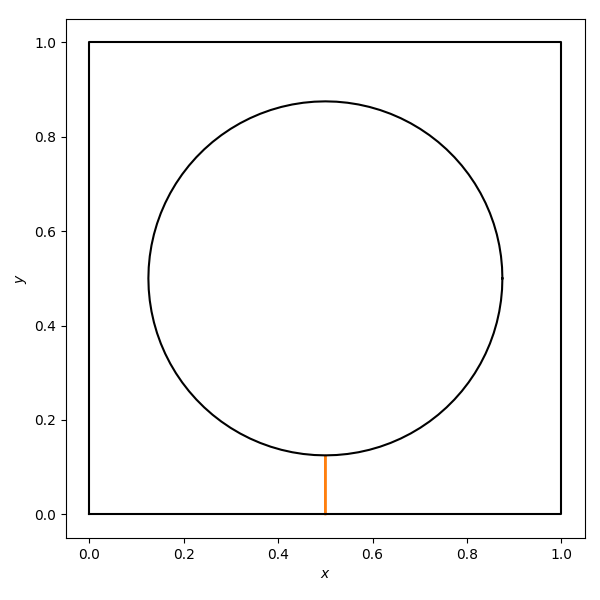
\includegraphics[width=1.0\textwidth]{sinai2b.png}
           %\caption{$R=3/8$.}
           \label{fig:pot1a}
       \end{subfigure}
       \begin{subfigure}[b]{0.43\textwidth}
          \hspace*{0mm}
           \centering
           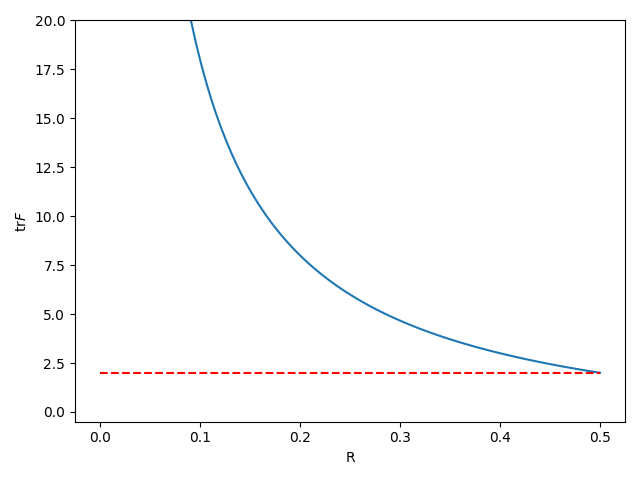
\includegraphics[width=1.0\textwidth]{sinai2b_1.png}
           %\caption{$R=3/8$.}
           \label{fig:pot1a}
       \end{subfigure}
\end{figure}
\begin{equation}
\begin{split}
F =& F_{odb_2} F_{prost_2} F_{odb_1} F_{prost_1} \\
 =& 
\begin{bmatrix}
-1 & 0\\
\frac{2}{-R} & -1
\end{bmatrix}
\begin{bmatrix}
1 & l\\
0 & 1
\end{bmatrix}
\begin{bmatrix}
-1 & 0\\
0 & -1
\end{bmatrix}
\begin{bmatrix}
1 & l\\
0 & 1
\end{bmatrix} \\
=&
\begin{bmatrix}
1 &2 l\\
\frac{2}{R} & 1 + \frac{4 l}{R}
\end{bmatrix} \\
=&
\begin{bmatrix}
1 & 1-2 R\\
\frac{2}{R} & 1 + \frac{2}{R} - 4
\end{bmatrix}
\end{split}
\end{equation}

\begin{equation}
\text{tr}F = -2(1 - \frac{1}{R})
\end{equation}




\item $\psi_{1,2,3,4} = \frac{\pi}{4}$, $\rho_{1,2,3,4} = \infty$, $R<\frac{\sqrt{2}}{4}$
\begin{figure}[H]
       \centering
       \hspace*{-0mm}
       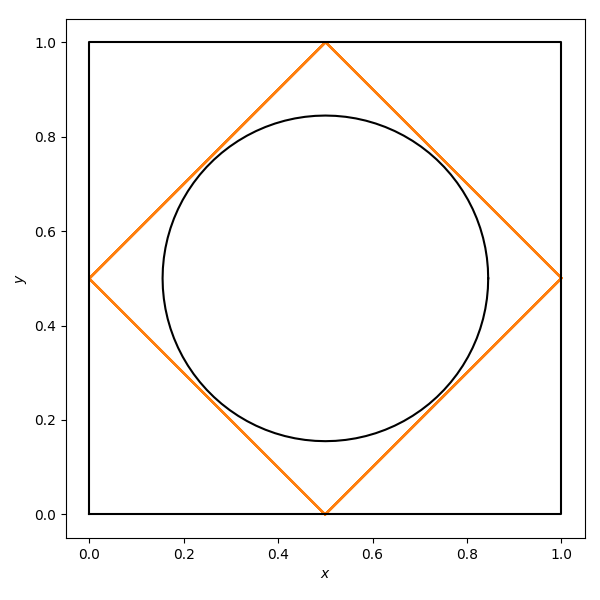
\includegraphics[width=5cm]{sinai2c.png}
       %\caption{Bouncing ball 1.}
       \label{fig:}
\end{figure}
\begin{equation}
\begin{split}
F =& F_{odb_4} F_{prost_4} F_{odb_3} F_{prost_3} F_{odb_2} F_{prost_2} F_{odb_1} F_{prost_1} \\
 =& 
\begin{bmatrix}
-1 & 0\\
0 & -1
\end{bmatrix}
\begin{bmatrix}
1 & l\\
0 & 1
\end{bmatrix}
\begin{bmatrix}
-1 & 0\\
0 & -1
\end{bmatrix}
\begin{bmatrix}
1 & l\\
0 & 1
\end{bmatrix}
\begin{bmatrix}
-1 & 0\\
0 & -1
\end{bmatrix}
\begin{bmatrix}
1 & l\\
0 & 1
\end{bmatrix}
\begin{bmatrix}
-1 & 0\\
0 & -1
\end{bmatrix}
\begin{bmatrix}
1 & l\\
0 & 1
\end{bmatrix} \\
=&
\begin{bmatrix}
1 & 4 l\\
0 & 1
\end{bmatrix}
\end{split}
\end{equation}

\begin{equation}
\text{tr}F = 2
\end{equation}




\item $\psi_{i} = \frac{\pi}{4}$, $\rho \in \{- R,\infty\}$
\begin{figure}[H]
\hspace*{18mm}
       \begin{subfigure}[b]{0.32\textwidth}
          \hspace*{0mm}
           \centering
           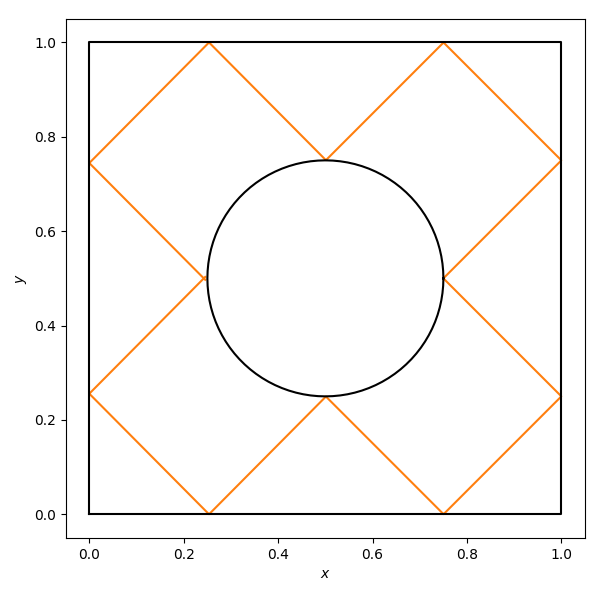
\includegraphics[width=1.0\textwidth]{sinai2d.png}
           %\caption{$R=3/8$.}
           \label{fig:pot1a}
       \end{subfigure}
       \begin{subfigure}[b]{0.43\textwidth}
          \hspace*{0mm}
           \centering
           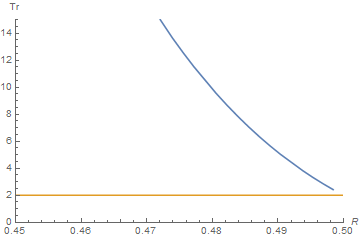
\includegraphics[width=1.0\textwidth]{detelja.png}
           %\caption{$R=3/8$.}
           \label{fig:pot1a}
       \end{subfigure}
\end{figure}
\begin{equation}
\begin{split}
F =& F_{odb_{12}} F_{prost_{12}} \dots F_{odb_2} F_{prost_2} F_{odb_1} F_{prost_1} \\
 =& \dots  \; Mathematica
\end{split}
\end{equation}

\begin{equation}
\text{tr}F > 2
\end{equation}
\end{itemize}
Seveda se pri manjših vrednostih $R$ pojavijo še druge periodične orbite, kot prikazuje slika \ref{fig:poinc}.
Na koncu predstavitve smo ugotovili, da s tako simulacijo dobimo precejšnjo napako.
Boljši način namesto numerične integracije med dvema odbojema je vsekakor iskanje naslednjega točnega presečišča z robom.
Artefakt tega sem tudi opazil pri zadnji periodični orbiti, ki se je po večjem številu iteracij zamaknila in prešla v kaos.
\end{document}